\documentclass[12pt]{article}
\usepackage{setspace}
%\setstretch{2}
\usepackage{color}  
\usepackage{hyperref}
\hypersetup{
	colorlinks=true, %set true if you want colored links
	linktoc=all,     %set to all if you want both sections and subsections linked
	linkcolor=blue,  %choose some color if you want links to stand out
	citecolor=red,
}
\usepackage{geometry}  
\geometry{letterpaper}      
\usepackage{graphicx}
\usepackage{amssymb}
\usepackage{amsmath}
\usepackage{mathrsfs}
\usepackage{appendix}
\usepackage{tikz}
\usepackage[numbers]{natbib}
\newcommand{\red}[1]{\textcolor{red}{#1}}
\newcommand{\blue}[1]{\textcolor{blue}{#1}}
\newcommand{\brown}[1]{\textcolor{blue}{#1}}
\newcommand{\green}[1]{\textcolor{green}{#1}}
\newcommand{\yellow}[1]{\textcolor{yellow}{#1}}
\usepackage{booktabs}   % professional-quality tables
\usepackage{multirow}
\usepackage{scrextend}
\usetikzlibrary{positioning}% To get more advances positioning options
\usetikzlibrary{arrows}% To get more arrow heads
\newtheorem{remark}{Remark}
\newtheorem{definition}{Definition}[section]
\newtheorem{proposition}{Proposition}[section] 
\newtheorem{property}{Property}[section]
\newtheorem{properties}{Properties}[section]
\newtheorem{assumption}{Assumption}[section]
\newtheorem{theorem}{Theorem}[section]
\newtheorem{corollary}{Corollary}[section]
\newtheorem{lemma}{Lemma}[section]
\newtheorem{example}{Example}[section]
\newenvironment{proof}{{\noindent\it Proof}\quad}{\hfill $\square$\par} 
\numberwithin{figure}{section}
\numberwithin{equation}{section}
\usepackage{algorithm}
\usepackage{algorithmic}
\usepackage{bm}
\usepackage{stmaryrd}
\usepackage{pdfpages}
\title{Literature Review on Shale Gas Modeling and Numerical Simulation}{
\date{}
\author{Boqian Shen}

\begin{document}
\maketitle
\tableofcontents
\section{Introduction}
\begin{figure}[H]
\centering
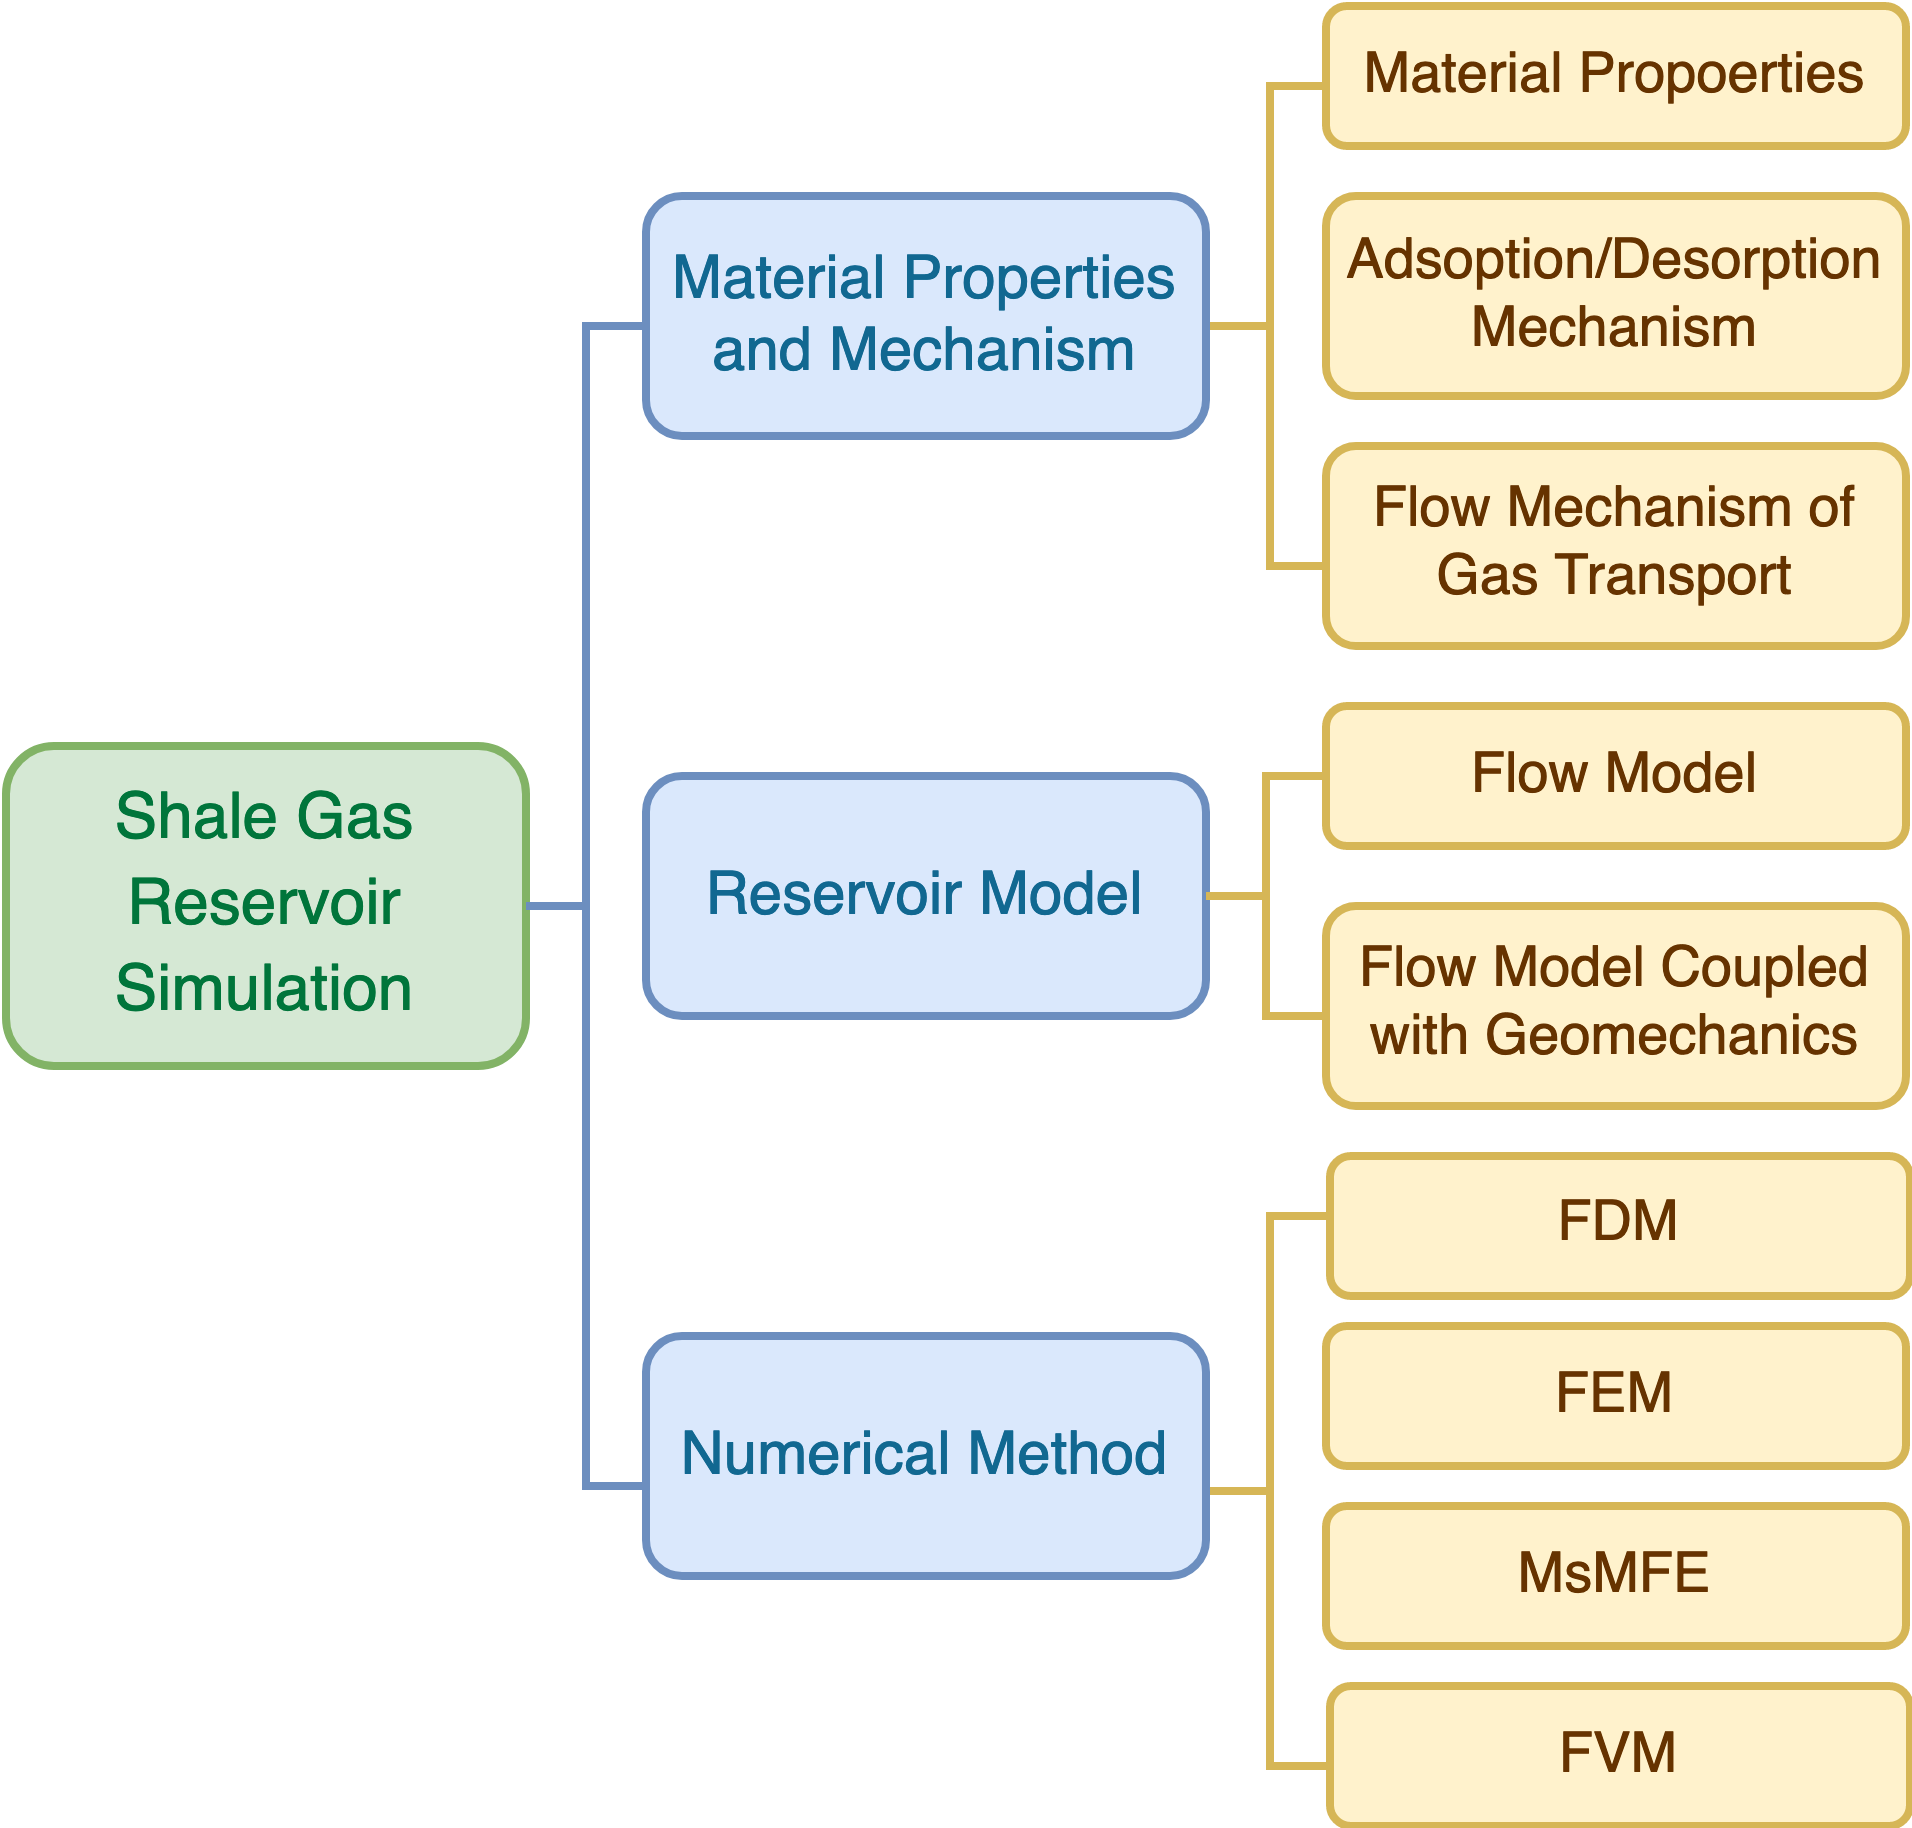
\includegraphics[width=0.8\linewidth]{pictures/shale_gas_main_structure.png}
%\caption{}
\label{fig:shale_gas_simulation_main_structure}
\end{figure}
\section{Modeling}
\section{Numerical Method}
\section{Review Notes}
%\input{shizhe_li}
\subsubsection{Zhang, Tao, Shuyu Sun, and Hongqing Song. "Flow mechanism and simulation approaches for shale gas reservoirs: A review."  \citep{zhang2019flow}}
\begin{itemize}
\item Material’s Properties
\begin{itemize}
\item Permeabilit is alwasy relatively low, less than 1 md.
\item The stresssensitive parameters, including organic richness, porosity, thickness and lateral extent, can vary significantly with in stress changes.
\end{itemize}
\item Adsorption/Desorption Mechanism
\begin{itemize}
\item There are three states of has reserved in shale reservoir: free gas, adsorbed gas(main state 20-80\%) and dissolved gas.
\item With the decrease in pressure, adsorbed gas sill become free gas in the early period of exploitation.
\item methane adsorption
\item adsorption capacity (TOC total organic carbon, shale contains high orgnic matter→ high gas adsorption)
\item gas adsorption process can be described by various isotherm models: Langmuir’s type model (simplest and effective), Freundlich-type model, Langmuir–Freundlich-type model, D-R-type model, BET-type model and Toth-type models.
\item Multi-component adsorption mechanisms,composition of varieties of hydrocarbons (C2+) and subsequently high total organic content(TOC)
\end{itemize}
\item Flow Mechanisms of Gas Transport in Shale Gas Reservoir
\begin{itemize}
\item Flow Regime
\begin{itemize}
\item pore size ranging from macroscale (>1mm) to nanoscale (<100 nm)
\item Kn → flow regime → governing equation+boundary condition
\end{itemize}
\item  Based on the Knudsen numbers (Kn), the flow mechanism can be classified as two categories:
\begin{itemize}
\item molecular dynamics for shale gas transportation: adsorption, diffusion, displacement and other mechanisms
\item lattice Boltzmann method : slippage, Knudsen diffusion, and apparent permeability correction(to improve Darcy’s law where matrix with low velocities and freactures with high velocities.
\item Apparent Permeability Correction
\item Improved Darcy Model in Fractures
\end{itemize}
\end{itemize}
\item Reservoir Models (reservoir-scale Gas flow  simulation)
\begin{itemize}
\item Flow model
\begin{itemize}
\item porous media: inter-particle and intra-particle(organic matter pores within kerogen and mineral particles) pores
\item Kerogen is the place gas adsorbs on the wall and dissolves within it
\item Gas is considered as wetting phase
\item Four types of organic matter: hydraulic fractures, natural fractures, kerogen (organic matrix) and inorganic matter, with the derease in pore size
\item Another classification: organic porosity, inorganic porosity, natural fractures and hydraulic fractures
\item single porosity for shale gas simulation: Multiple interacting continua (MINC) and explicit fracture modeling
\item for different pore sizes such as dual porosity model, connection between nanopores and micropores in organic matter has to be considered: Darcy’s law (limited, low permeability) and Fickian diffusion should be considered
\end{itemize}
\item Flow Model Coupled with Geomechanics
\begin{itemize}
\item A popular trend is to use geomechanism with flow model for gas production simulation, otherwise the production will be overestimated, since the production is sensitive to fracture aperture changes
\item pressure, deformation, linear elasticity, nonlinear elasticity(for better estimation on permeability)
\end{itemize}
\end{itemize}
\item Numerical Approaches
\begin{itemize}
\item - Finite Difference Method (FDM)
efficiency and simplicity, with rectangular and triangular grid, uniform and non-uniform meshes, cartesian and curvilinear coordinates, 1D to 3D.  Firoozabadi 1999
 
\item Finite Element Method (FEM)
more arrutate, unstructured meshes (fracture)
    
\item Multiscale mixed finte element (MsMFE) method 
The main process is to make this method as geometrically flexible as possible and developing coarsening strategies that semiautomatically adapt to barriers, channels, faults and wells in a way that ensures good accuracy for a chosen level of coarsening.
\item AMG
\item Finite Volume method FVM
more easily implemented with unstructured grids
\item Fast marching method (FMM)
\end{itemize}
\end{itemize}

%\input{chensong_zhang}
%\input{li_zhao}

%\section*{References}
\bibliographystyle{plain}
\bibliography{ref}
\end{document}
